\documentclass{beamer}

\newcommand{\ket}[1]{\left|#1\right\rangle}
\newcommand{\op}[1]{\boldsymbol{\mathit{#1}}}
\newcommand\blfootnote[1]{%
  \begingroup
  \renewcommand\thefootnote{}\footnote{\tiny #1}%
  \addtocounter{footnote}{-1}%
  \endgroup
}
\usepackage{booktabs}
\usepackage{bbold} 
\usepackage{xcolor} 
\usepackage{color}
\usepackage{dsfont}
\usepackage[english]{babel}
\usepackage[latin1]{inputenc}
\usepackage{times}
\usepackage{tabularx}
\usepackage{multirow}
\usepackage{tikz}
\usepackage[T1]{fontenc}
\usepackage{xfrac}
\usepackage{graphicx}
\usepackage{mathtools}
\usepackage{physics}
\DeclareGraphicsRule{.ai}{pdf}{.ai}{}

\mode<presentation>
{
	\usetheme{Singapore}
	\usecolortheme{dove} %% Grigio
	\setbeamercovered{transparent}
}


%\setbeamertemplate{footline}[frame number] 
\expandafter\def\expandafter\insertshorttitle\expandafter{%
  \insertshorttitle\hfill%
  \insertframenumber\,/\,\inserttotalframenumber}

\setbeamertemplate{navigation symbols}{} %no nav symbols
\setbeamertemplate{itemize item}{}
\setbeamertemplate{headline}{}

\title[]{Photon-number and timing resolution of a near-IR continuous-wave source with a transition edge sensor \break IPS 2017}
% \subtitle{}

\author[A. Cer{\`e}] % (optional, use only with lots of authors)
{Jianwei Lee*, Lijiong Shen, Brenda Chng, Alessandro Cere, Christian Kurtsiefer}

% \pgfdeclareimage[height=1.3cm]{university-logo-full}{Images/logo}
\institute[CQT] % (optional, but mostly needed)
{
%   \inst{1}%
\begin{columns}
  \column{.4\textwidth}
  \begin{center}    
    \includegraphics[width=0.8\textwidth]{images/NUS_Logo.ai}
    \end{center}  
  \column{.5\textwidth}
  \begin{center}
  	 \includegraphics[width=\textwidth]{images/CQTLogo.ai}\\
		 Quantum Optics Group	
  \end{center}
\end{columns}
}

\date{}
% \date{
%   \begin{center}
%   IPS 2015\\
%   4 Mar \\
%   01.50pm $-$ 02.05pm
%   \end{center}
% }
% \date[]{04/03/2015} % (optional, should be abbreviation of conference name)
%{Centre for Quantum Technology - UKZN}
\subject{Pulse Fitting}
% This is only inserted into the PDF information catalog. Can be left
% out. 

%\pgfdeclareimage[height=0.5cm]{university-logo}{images/cqtblue_notext}
%\logo{\pgfuseimage{university-logo}}

% \AtBeginSection[]
% { \addtocounter{framenumber}{-1}
%   \begin{frame}<beamer>[plain]
%     \frametitle{Outline}
%     \tableofcontents[currentsection,currentsubsection]
%   \end{frame}
% }


\begin{document}

\begin{frame}[plain]
  \setcounter{framenumber}{0}
  \titlepage
\end{frame} 

\begin{frame}\frametitle{Motivation}
  \begin{center}
      \begin{block}{Measure 2nd-order correlation function with a single detector}
      \begin{itemize}
        \item Avoids spatial multiplexing of Hanbury-Brown-Twiss
        \item Applicable to Satellites \blfootnote{J.W. Fowler, ApJS \textbf{219} 35 (2015)} 
      \end{itemize}
      \end{block}
    \end{center}
\end{frame}

\begin{frame}\frametitle{Outline}
  \begin{itemize}
    \item Transition-Edge Sensor \& Setup
    \item Photon-Number Resolution
    \item Time-of-Arrival Estimation
    \item 2nd-Order Correlation of Continuous Source
  \end{itemize}
\end{frame}

\begin{frame}\frametitle{Transition-Edge Sensor}
  \begin{center}
      \begin{itemize}
        \item Photon-Number Resolving
        \item Near unit Efficiency
        \item Long Recovery Time ($\approx 2 \mu s$) limits flux detection rates\
      \end{itemize}
    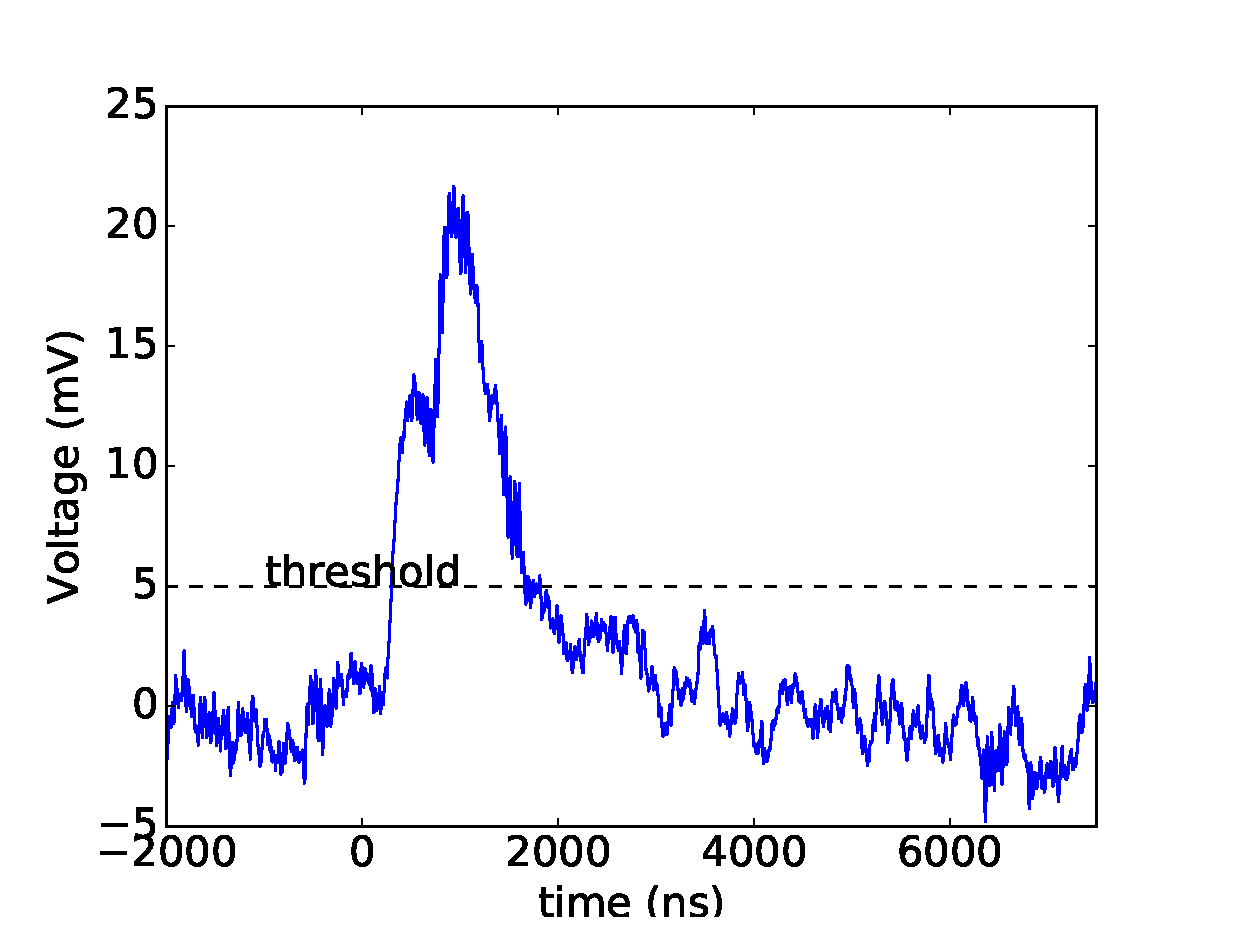
\includegraphics[width=0.7\textwidth]{images/comparator/overlapping_pulses.eps}
    \end{center}
\end{frame}

\begin{frame}\frametitle{Transition-Edge Sensor}
    
  Photon absorbed $\rightarrow$ Temperature increases $\rightarrow$ Resistance increases

  \begin{columns}
  \column{.5\textwidth}
    \begin{center}
    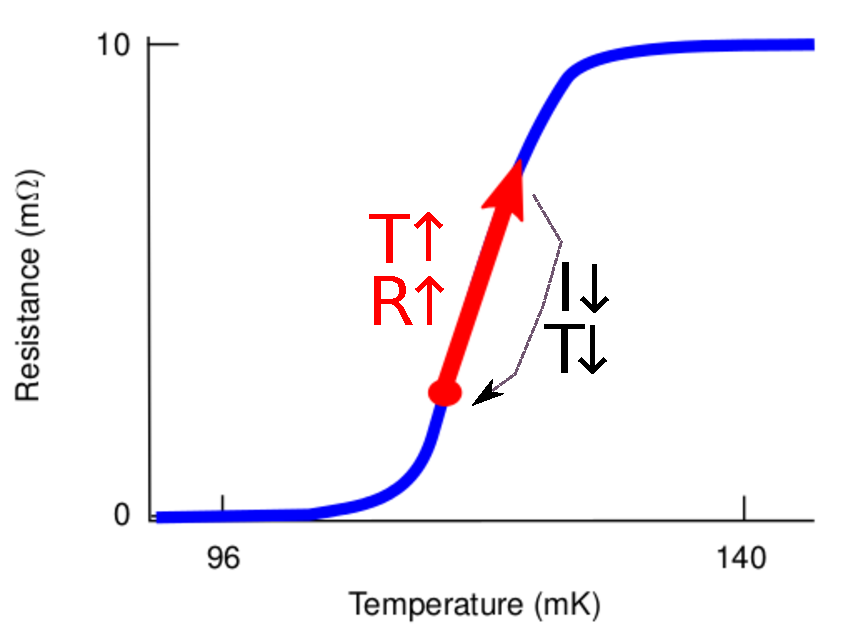
\includegraphics[width=1.2\linewidth]{images/tes_principle/TES.pdf}
    \end{center}
  \column{.5\textwidth}
    \begin{center}
    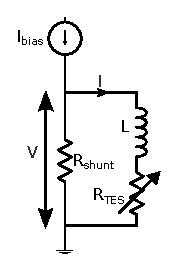
\includegraphics[width=0.5\linewidth]{images/electronics/tes_only_electronics.eps}
    \end{center}
  \end{columns}
\blfootnote{A.E.Lita, Proc. SPIE 7681, Adv Photon Counting Techniques IV, 76810D (2010)}
\end{frame}

\begin{frame}\frametitle{Photon Number Discrimination}
  \begin{center}
  Light source: Pulsed Laser Diode\\
  Pulse Area $\propto$ Photon Number
  \begin{columns}
    \column{.6\textwidth}
        \begin{center}
          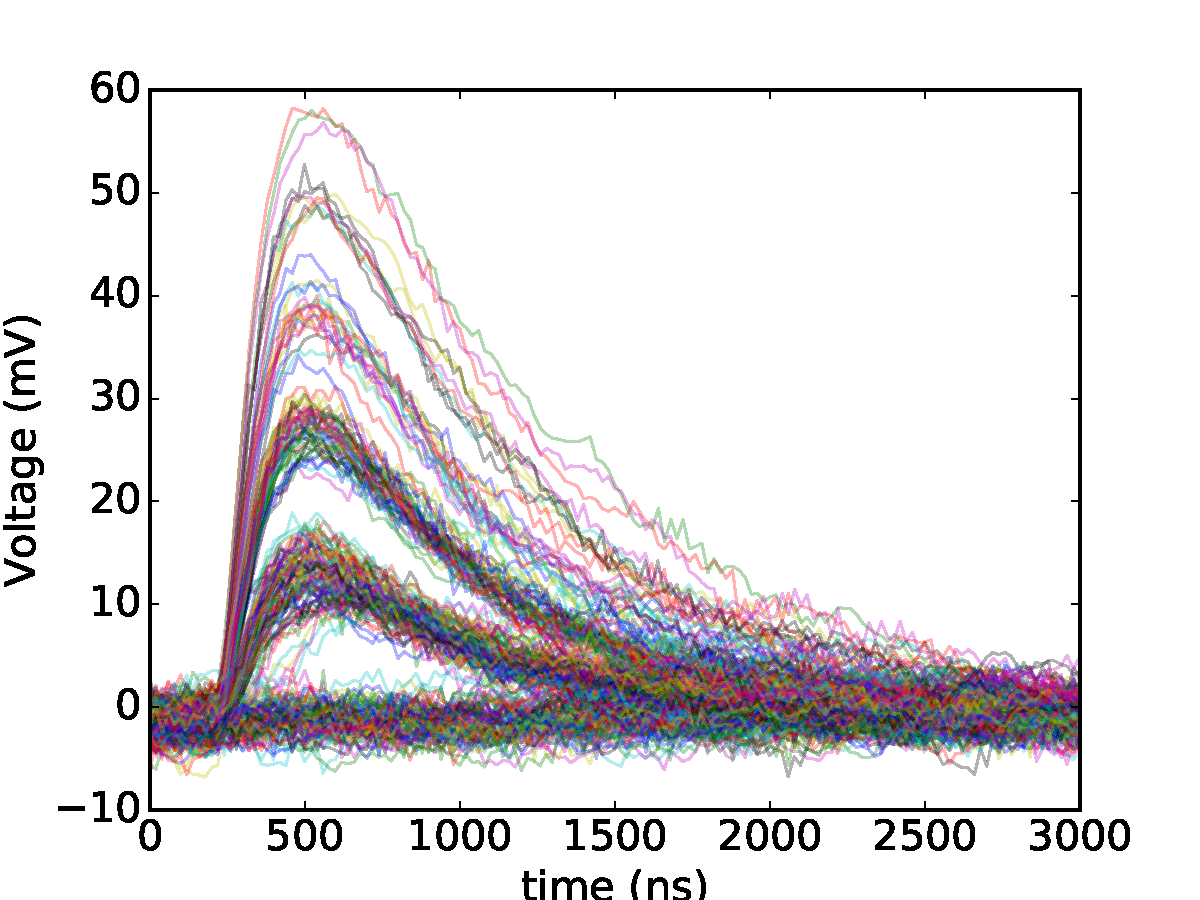
\includegraphics[width=1\textwidth]{images/persistence_plot/persistence.pdf}
        \end{center}
    \column{.6\textwidth}
        \begin{center}
          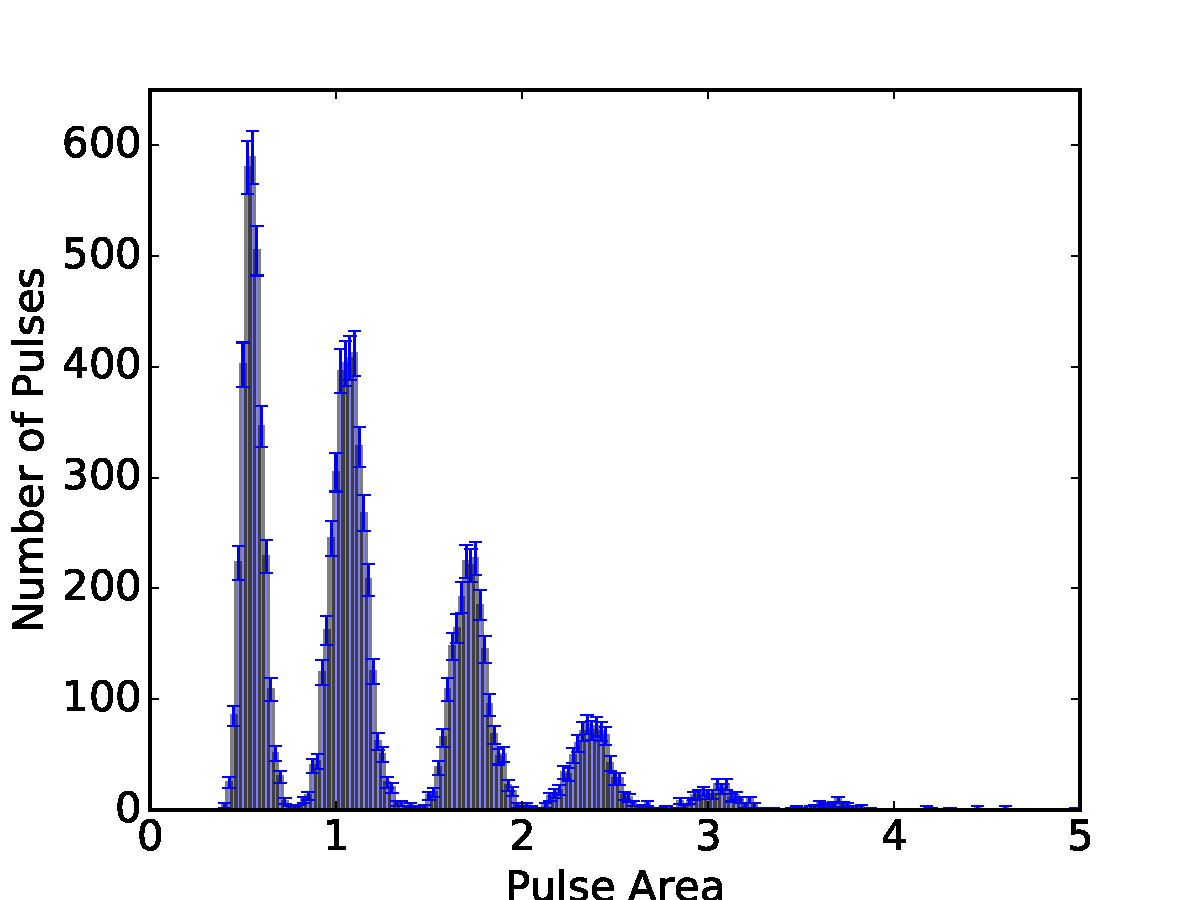
\includegraphics[width=1\textwidth]{images/area_histogram_single_diode_pulse/area_histo.pdf}
        \end{center}
    \end{columns}
  \end{center}
\end{frame}
\begin{frame}\frametitle{Pulse Identification for Continuous Source}
  \begin{center}
  \begin{itemize}
  \begin{center}
  \item Discard Incomplete Pulses at Edges
  \item Limit Background Noise
  \end{center}
  \end{itemize}
  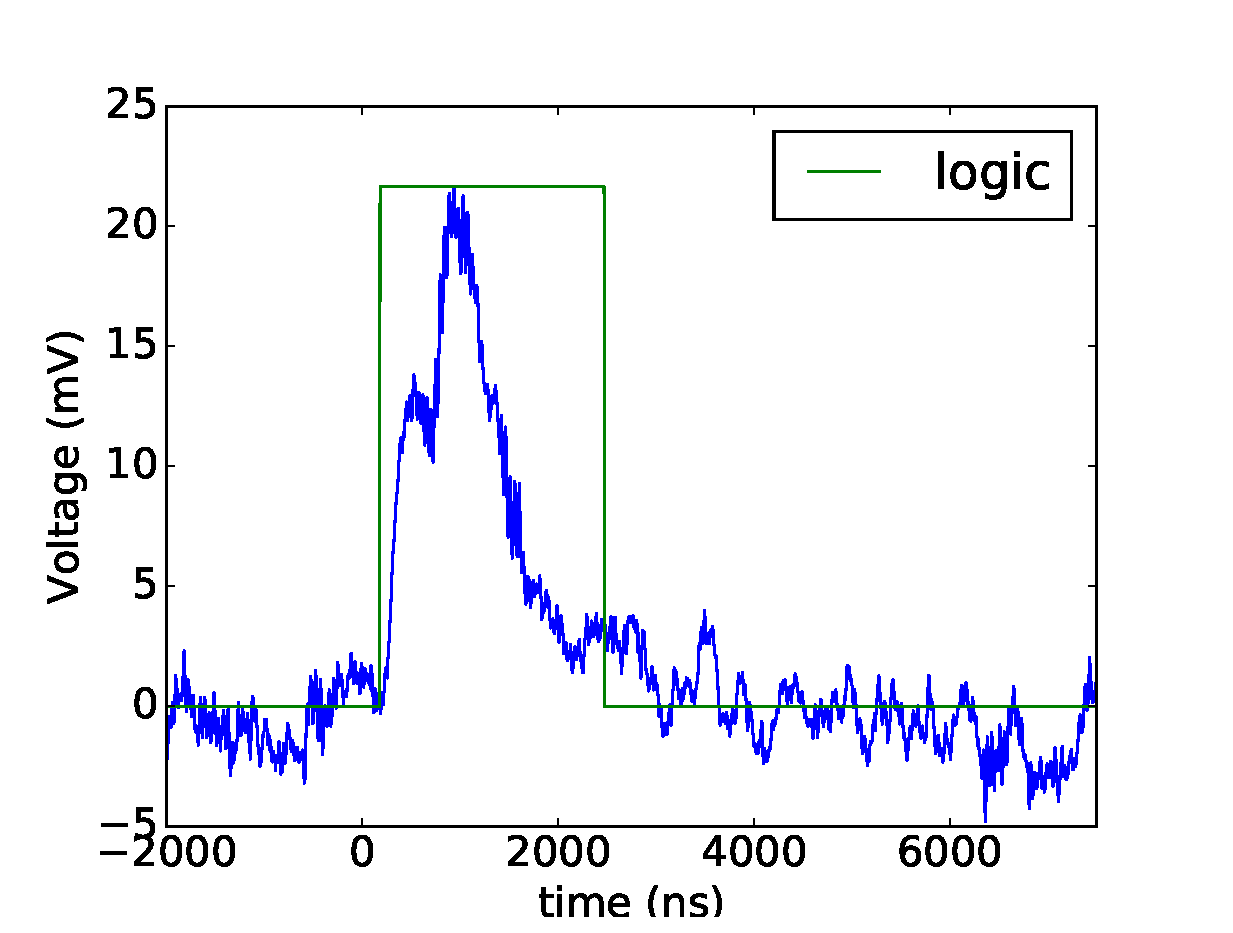
\includegraphics[width=0.7\textwidth]{images/comparator/comparator_at_500ns.eps}
  \end{center}
\end{frame}

\begin{frame}\frametitle{Photon Number Resolution\\(Continuous Source)}
  \begin{center}
  \begin{columns}
    \column{.5\textwidth}
        \begin{center}
        NO Pulse Identification
          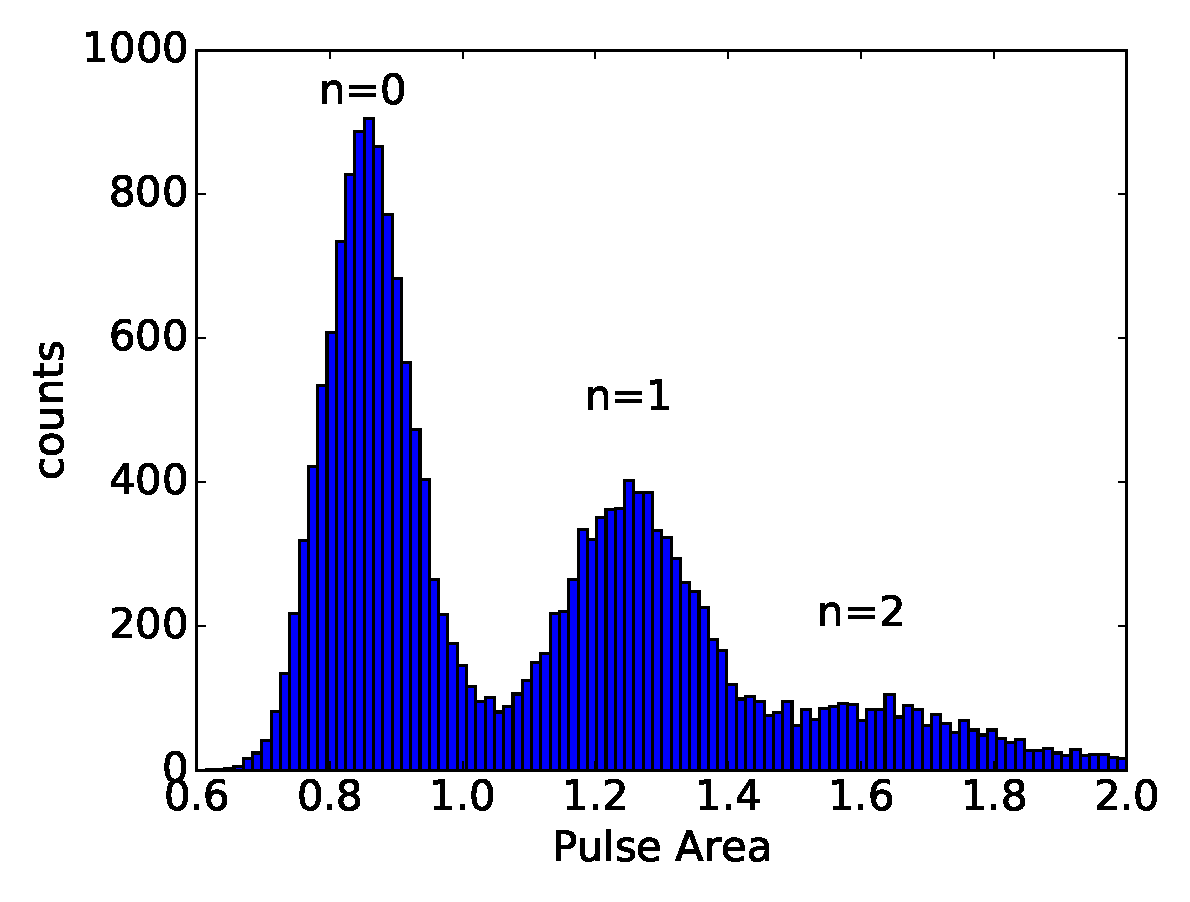
\includegraphics[width=1\textwidth]{images/area_distribution/area_abs_histo.eps}
        \end{center}
    \column{.5\textwidth}
        \begin{center}
        Pulse Identification
          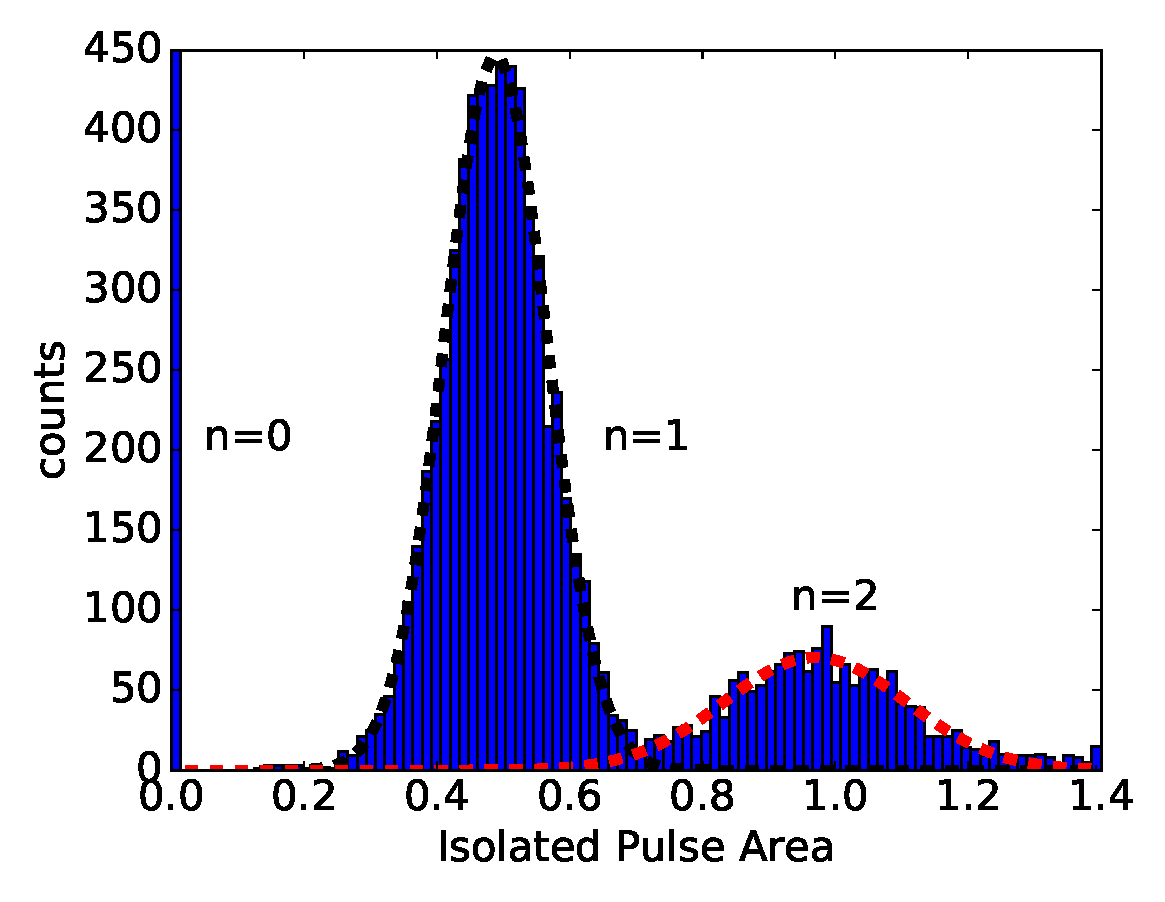
\includegraphics[width=1\textwidth]{images/area_distribution/area_windowed_histo.eps}
        \end{center}
    \end{columns}
  \end{center}
\end{frame}
\begin{frame}\frametitle{Time-of-Arrival Estimation}
  \begin{center}
  \item \textcolor{gray}{Model:} $A_1S(t-t_1) + A_2S(t-t_2)$
  \begin{columns}
  \column{0.5\textwidth}
  \begin{enumerate}
    \item Select 2-photon signals (pulse area)
    \item Detect Pulse edges (filter + differentiate)
    \item 2 Edges
        \begin{itemize}
        \item Initialise using Pulse Edges Timings
        \item Least Squares Fit
        \end{itemize}
    \item 1 Edge
        \begin{itemize}
        \item Initialise using Pulse Region
        \item Monte-Carlo Markov Chain Fit
        \end{itemize}
  \end{enumerate}
  \column{0.5\textwidth}
  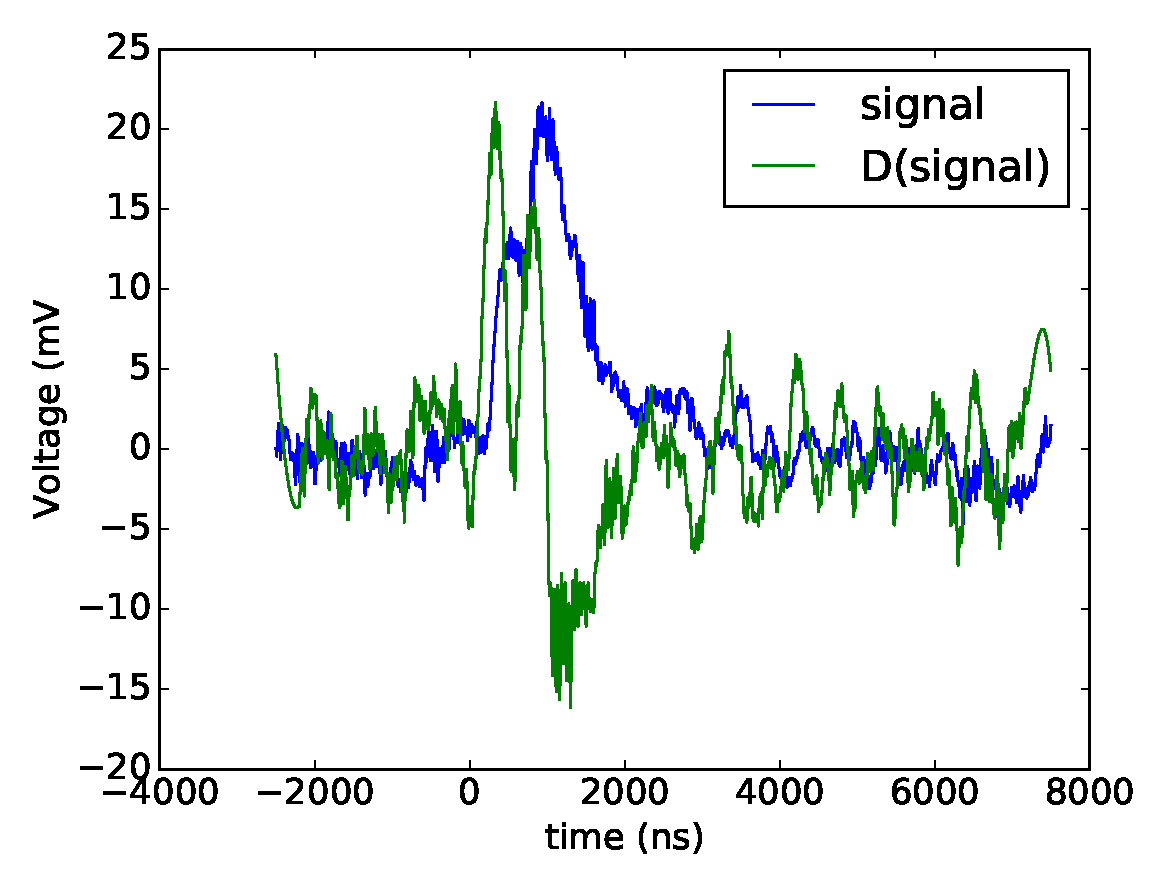
\includegraphics[width=\textwidth]{images/edge_detection_demonstration/edge_detection_by_diff.eps}
  \end{columns}
  \end{center}
\end{frame}

\begin{frame}\frametitle{Single-Photon Detection Model}
  \begin{center}
      % \begin{block}{}
      \begin{itemize}
      \begin{center}
        \item Select 5000 single-photon pulses
        \item Correct for Vertical \& Horizontal Offset
        \item Average
      \end{center}
      \end{itemize}
    % \end{block}
    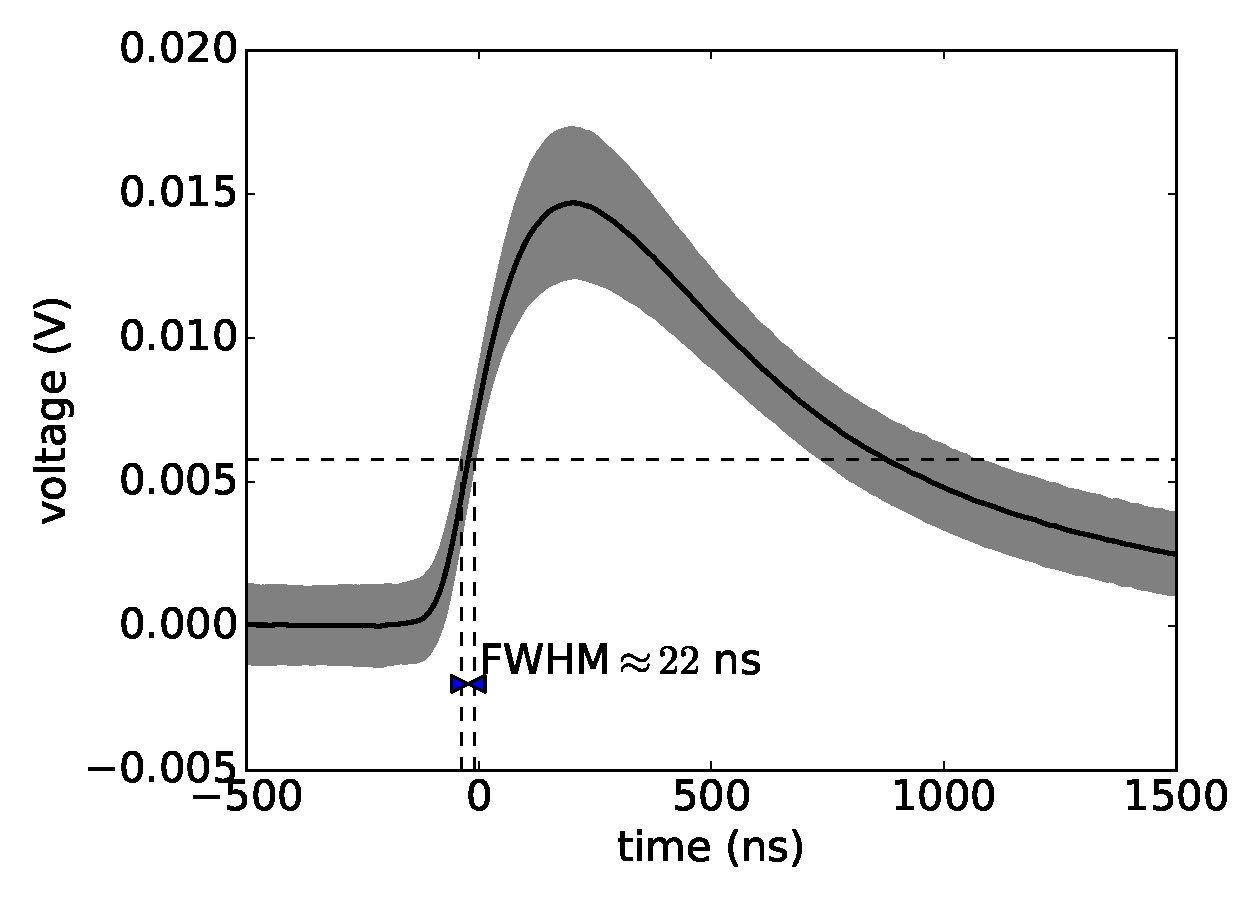
\includegraphics[width=0.7\textwidth]{images/intrinsic_jitter/jitter.eps}
    \end{center}
\end{frame}

\begin{frame}\frametitle{Self-Correlation $G^{(2)}$}
  \begin{center}
  CW Laser Diode
    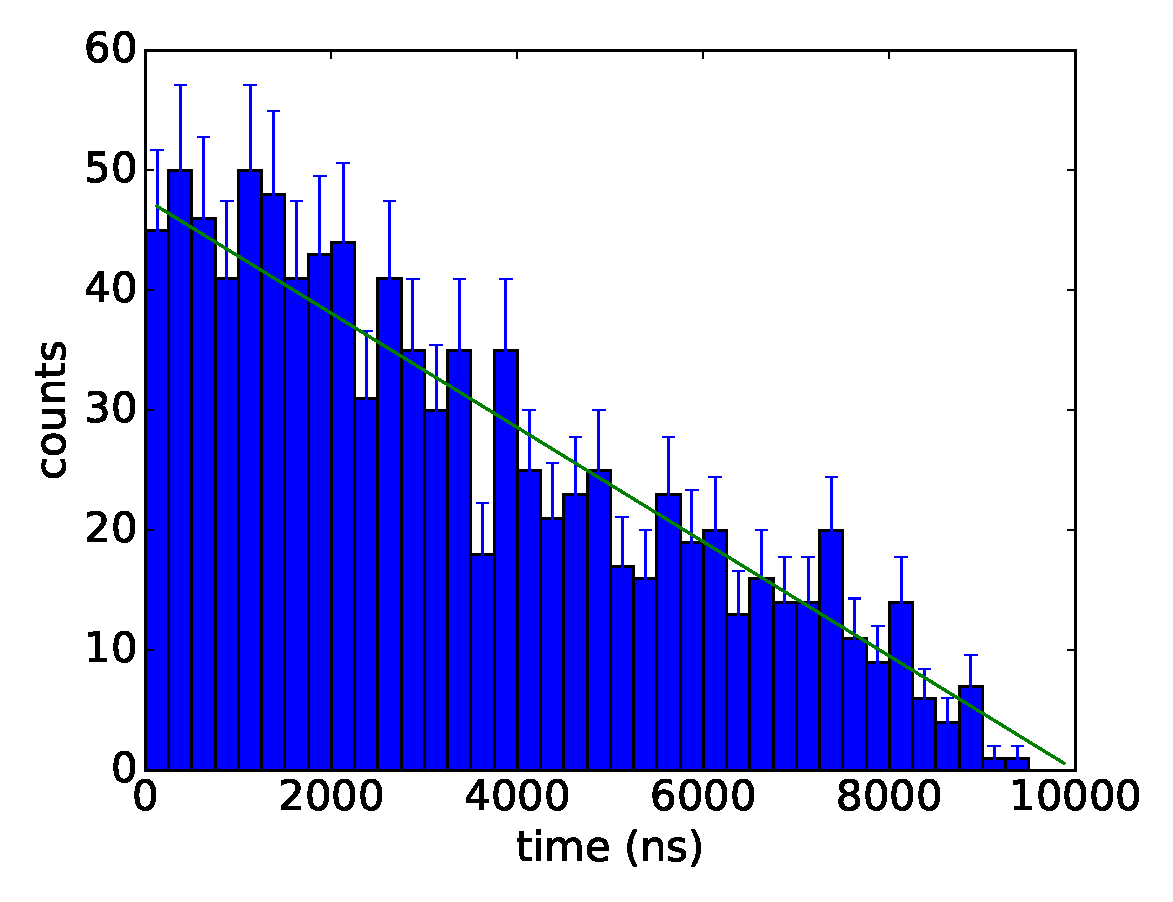
\includegraphics[width=\textwidth]{images/g2_cw_source/g2_cw_binsize_250ns.eps}
    \end{center}
\end{frame}

\begin{frame}\frametitle{Self-Correlation $G^{(2)}$}
  \begin{center}
  CW Laser Diode
    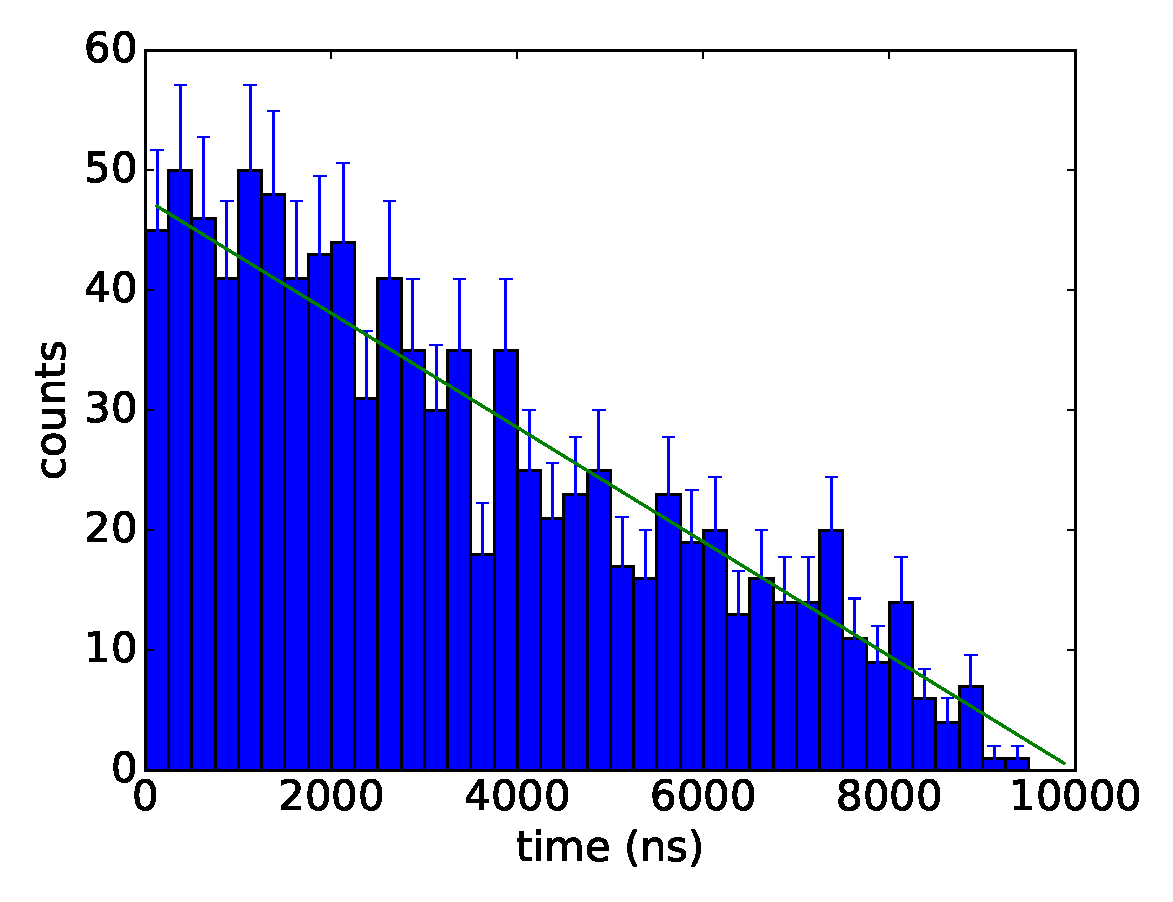
\includegraphics[width=\textwidth]{images/g2_cw_source/g2_cw_binsize_250ns.eps}
    \end{center}
\end{frame}

\begin{frame}\frametitle{Self-Correlation $G^{(2)}$\\Fit Accuracy}
  \begin{center}
  Light Source: Laser Diode Pulse Pairs
  \begin{columns}
  \column{.5\textwidth}
  \begin{center}
  Seperation > 200ns
    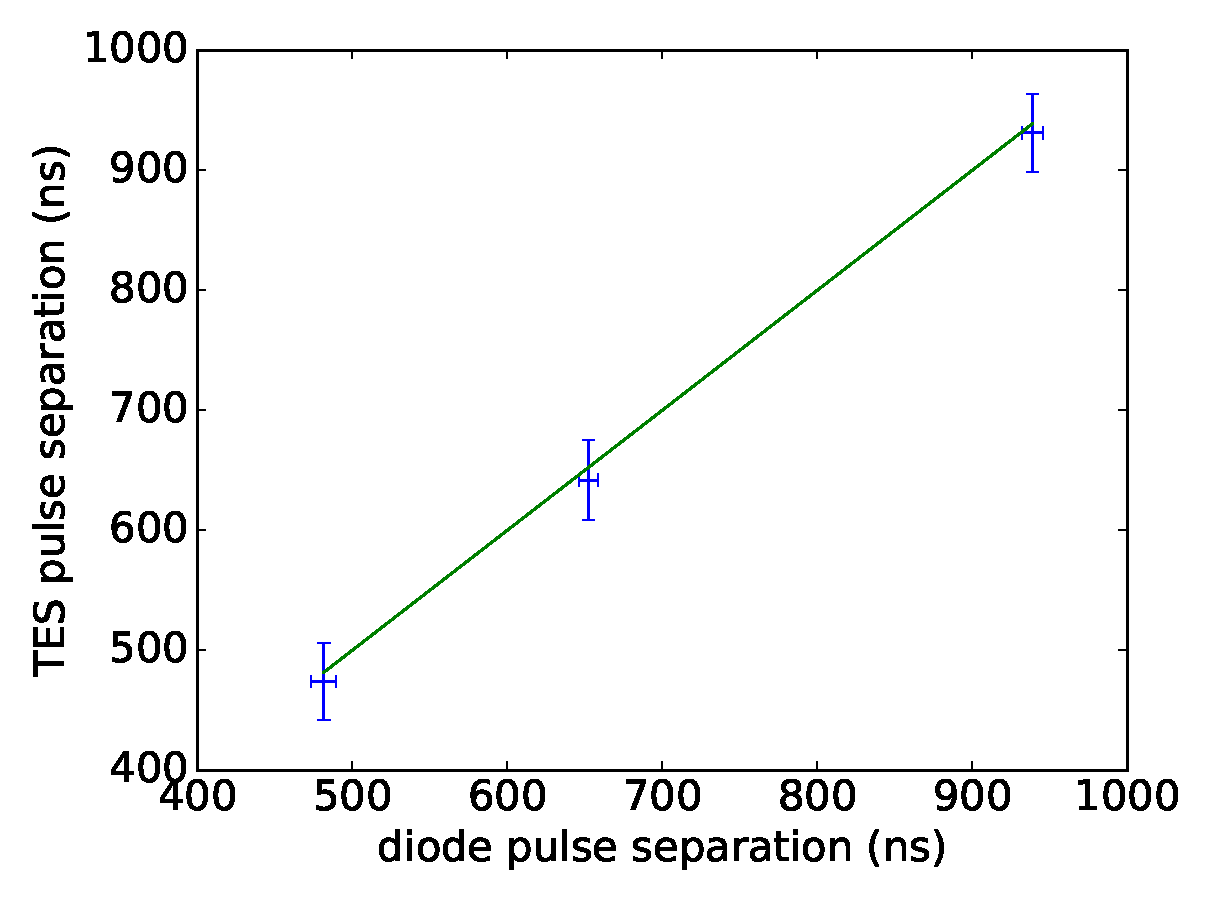
\includegraphics[width=\textwidth]{images/fit_accuracy/fitted_vs_actual_pulse_separation.eps}
  \end{center}
  \column{.5\textwidth}
  \begin{center}
  Seperation = 200ns
  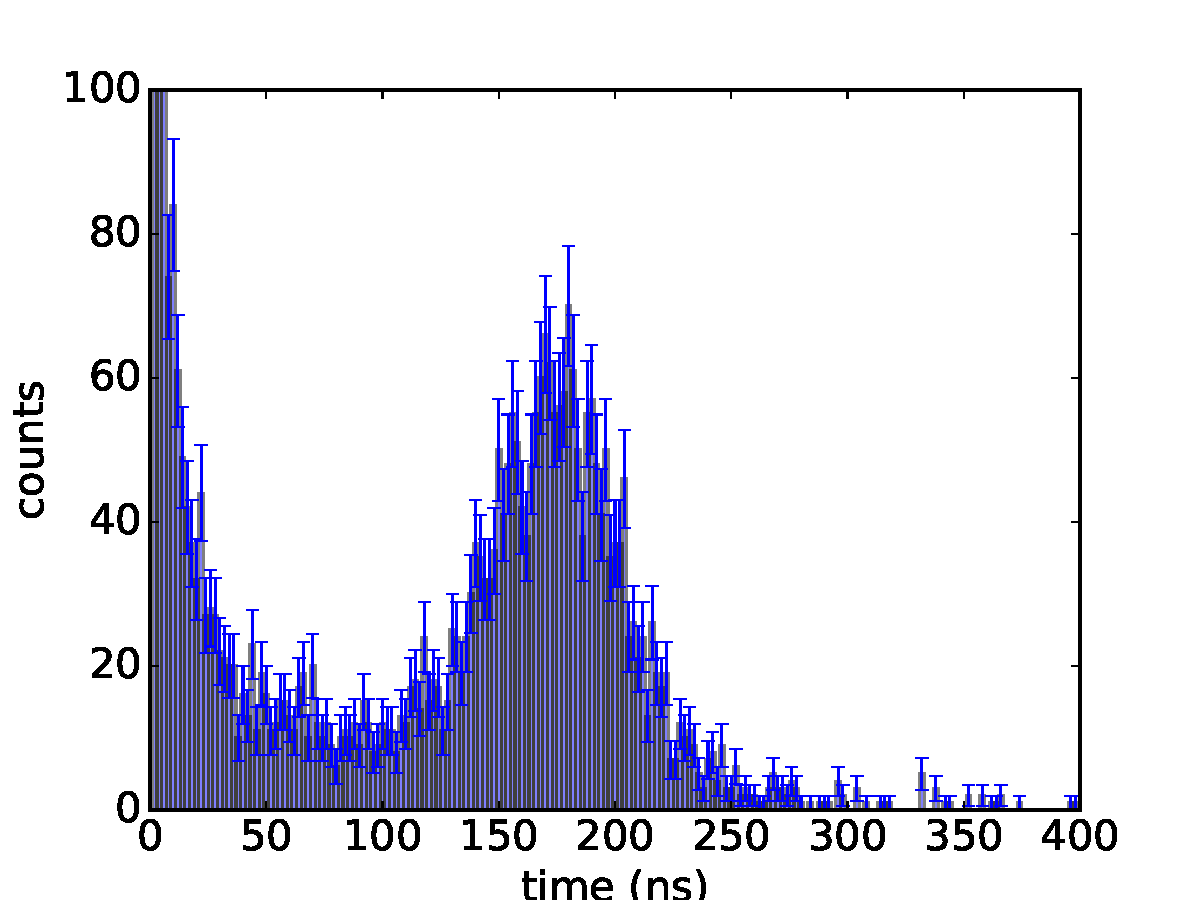
\includegraphics[width=\textwidth]{images/fit_accuracy/200ns/200ns_g2.pdf}
  \end{center}
  \end{columns}
  \end{center}
\end{frame}


\begin{frame}\frametitle{Conclusion}
  \begin{itemize}
  \item Timing Resolution $\approx 250~ns$
  \item Photon Number Resolution
  	\begin{itemize}
	  \item n = 0, 1 misidentification negigible
	  \item 1-photon event misidentified as 2-photon event: $0.8 \%$ 
	\end{itemize}
  \item Applications 
  	\begin{itemize}
  		\item Correlation measurements without spatial-mode multiplexing\blfootnote{J.W. Fowler, ApJS \textbf{219} 35 (2015)} 
  		\item Increased Photon Flux
  	\end{itemize}
  \end{itemize}
\end{frame}
\include{Q&A}
\end{document}
%EOF